\documentclass{standalone}

\usepackage{amsmath,amsfonts,amssymb,amsthm,mathtools} 
\usepackage{fontspec}            % пакет для подгрузки шрифтов
\setmainfont{Amiri}   % задаёт основной шрифт документа

% why do we need \newfontfamily:
% http://tex.stackexchange.com/questions/91507/
\newfontfamily{\cyrillicfonttt}{Amiri}
\newfontfamily{\cyrillicfont}{Amiri}
\newfontfamily{\cyrillicfontsf}{Burst My Bubble}
% Иногда тех не видит структуры шрифтов. Эти трое бравых парней спасают ситуацию и доопределяют те куски, которые Тех не увидел.

\usepackage{unicode-math}     % пакет для установки математического шрифта
\setmathfont{Asana Math}      % шрифт для математики

\usepackage{polyglossia}      % Пакет, который позволяет подгружать русские буквы
\setdefaultlanguage{russian}  % Основной язык документа
\setotherlanguage{english}    % Второстепенный язык документа

\usepackage{pgf,tikz,pgfplots}
\usetikzlibrary{arrows,calc}
\usepackage{relsize} 

\usepackage{graphicx} 
\usepackage{rotating}
\usepackage{xcolor}
\usepackage{color}

\newcommand{\BBig}{\fontsize{60}{60}\selectfont}

\definecolor{bl}{HTML}{333333}
\definecolor{latxlatx}{HTML}{434545}


\begin{document}

\centering
\begin{tikzpicture}[scale=1]


\node[inner sep=0pt] (russell) at (0,0) {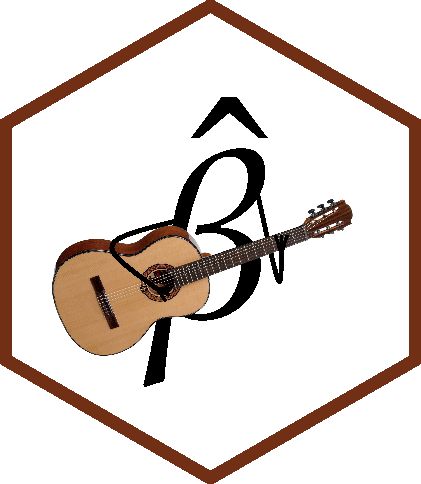
\includegraphics[height=5.08cm,width=4.39cm]{beta.pdf}};                             

\node[inner sep=0pt] (russell) at (2.5,-4.4) {
\includegraphics[height=5.08cm,width=4.39cm]{dummy_trap.pdf}}; 
   
\node[inner sep=0pt] (russell) at (-2.5,-4.4) {
\includegraphics[height=5.08cm,width=4.39cm]{zen.pdf}}; 

\node[inner sep=0pt] (russell) at (-5,0)   {
\includegraphics[height=5.08cm,width=4.39cm]{b+greater.pdf}};  

\node[inner sep=0pt] (russell) at (5,0) {
\includegraphics[height=5.08cm,width=4.39cm]{LaTeX-blud.pdf}};   
            
\node[inner sep=0pt] (russell) at (-2.5,4.4) {
\includegraphics[height=5.08cm,width=4.39cm]{LaTeX-logo.pdf}};

\node[inner sep=0pt] (russell) at (2.5,4.4) {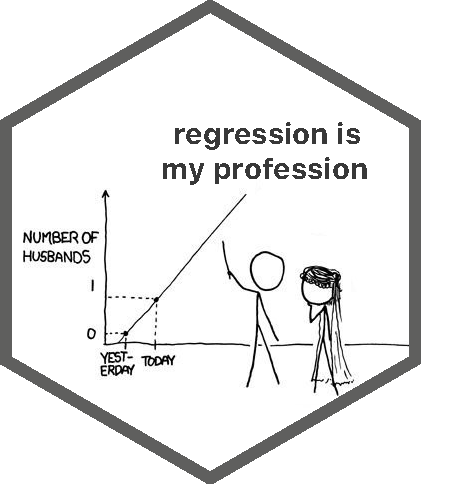
\includegraphics[height=5.08cm,keepaspectratio]{regression_is_my.pdf}};                
             

% Books 
\node[inner sep=0pt] (russell) at (0,-10) {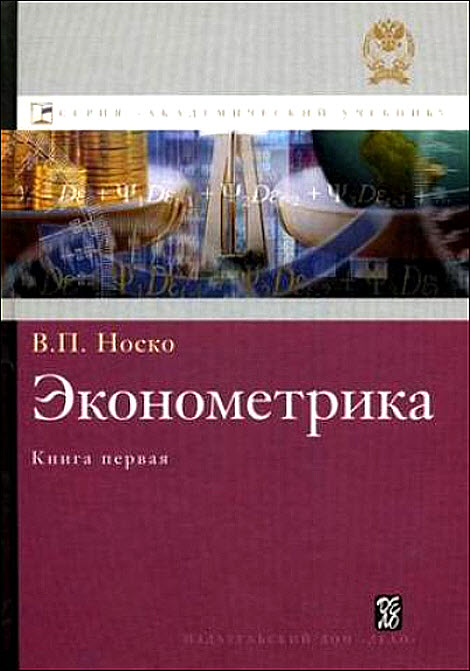
\includegraphics[height=4.39cm,keepaspectratio]{Nosko_1.jpg}};

\node[inner sep=0pt] (russell) at (-3.5,-10) {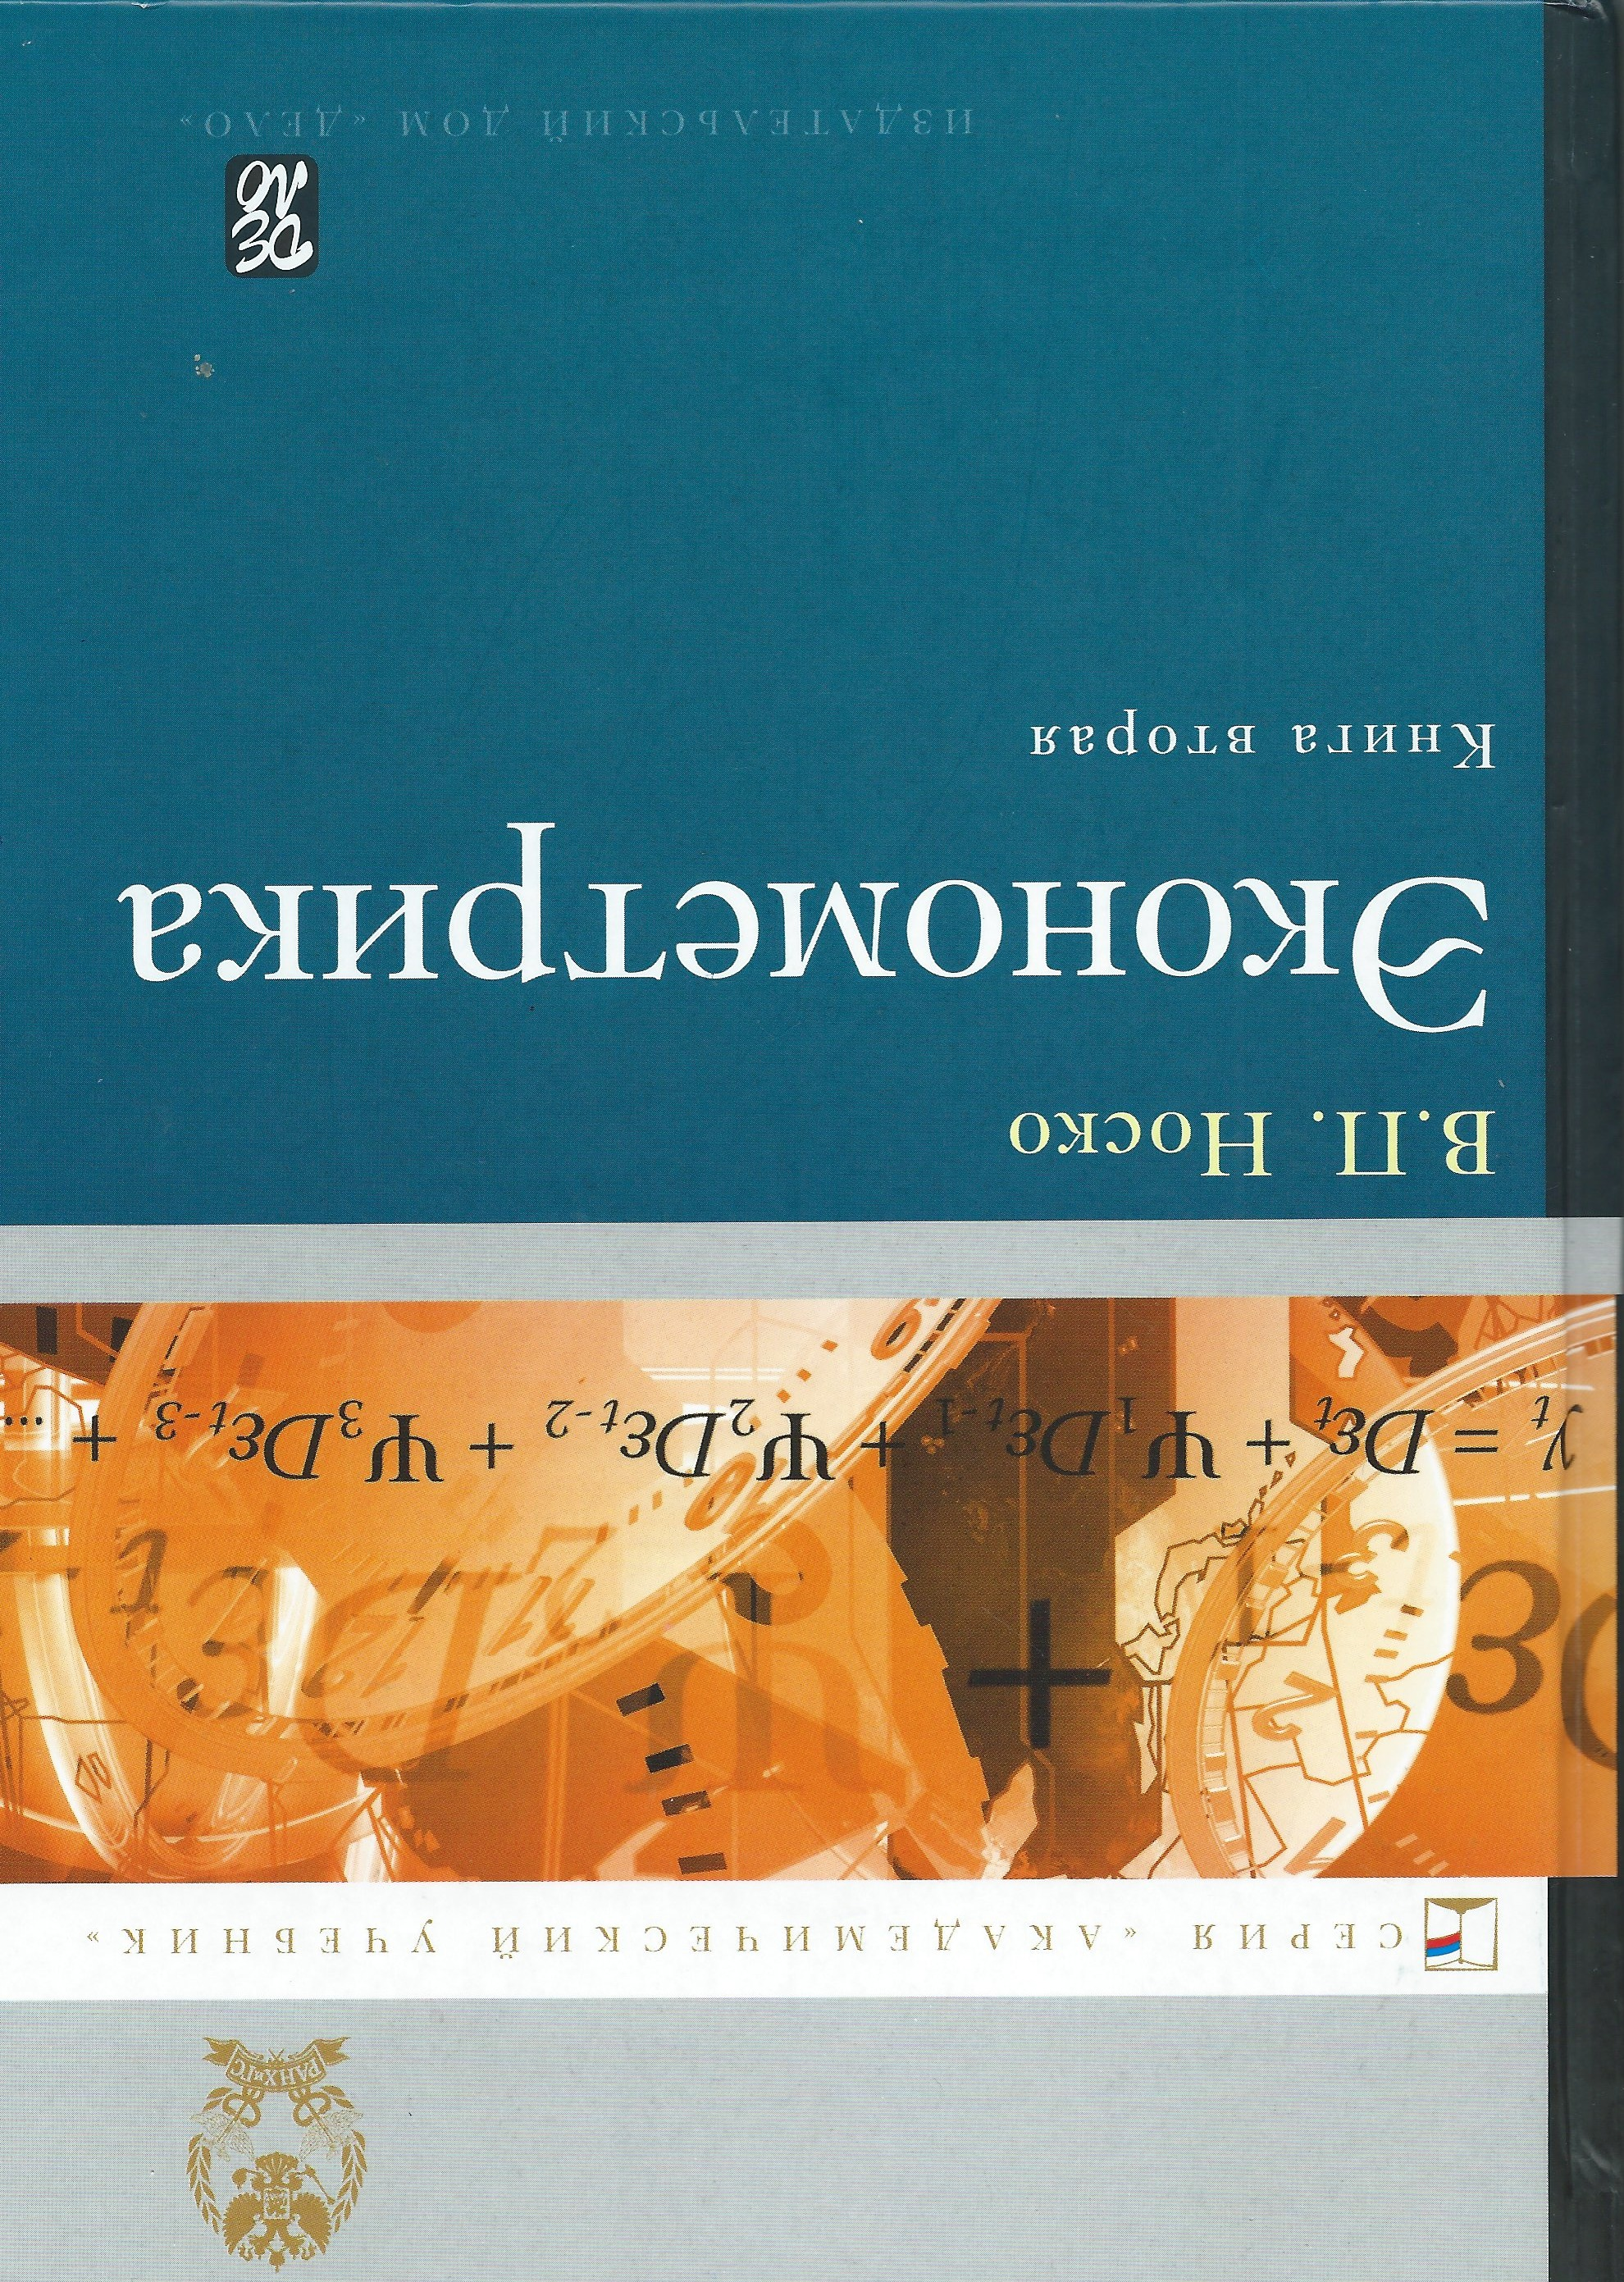
\includegraphics[height=4.39cm,keepaspectratio,angle=180]{Nosko_2.jpg}};    

\node[inner sep=0pt] (russell) at (3.5,-10) {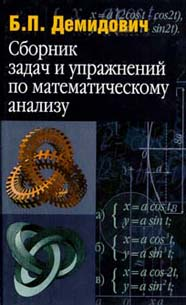
\includegraphics[height=4.39cm,keepaspectratio]{demidovich.jpg}};                

\hspace{1cm}

\end{tikzpicture}

%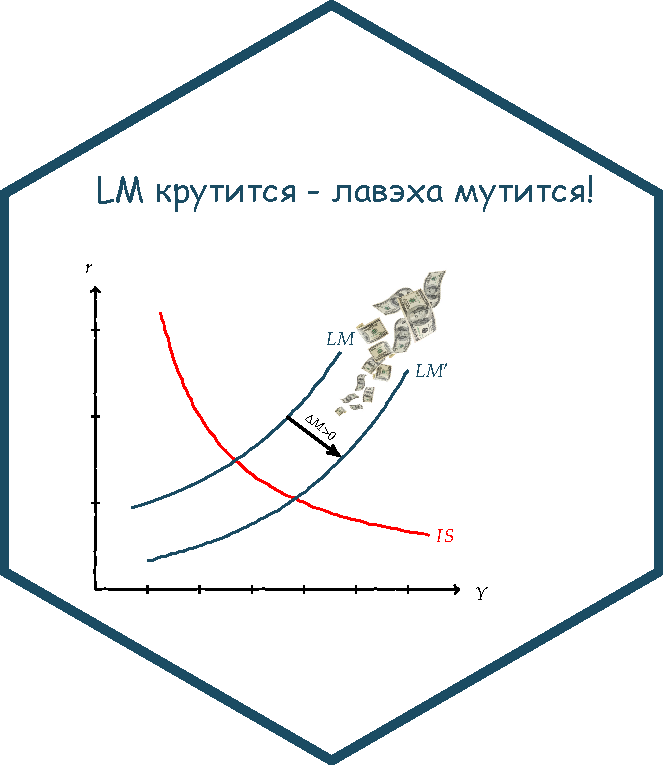
\includegraphics{ISLM.pdf}



\end{document}
